\documentclass[11pt]{article}
\usepackage[margin=0.75in]{geometry}
\geometry{a4paper}
\usepackage[T1]{fontenc} % Support Icelandic Characters
\usepackage[utf8]{inputenc} % Support Icelandic Characters
\usepackage{graphicx} % Support for including images
\usepackage{hyperref} % Support for hyperlinks
\usepackage{fancyhdr}

\usepackage{stix}
\usepackage{amsmath}
\usepackage{amssymb}
\usepackage{mathrsfs}
\usepackage{xcolor}
\usepackage{color}

\usepackage{booktabs}

\usepackage{mathtools}
\newcommand\myeq{\stackrel{\mathclap{\normalfont\mbox{d}}}{=}}
\newcommand\neweq{\stackrel{\mathclap{\normalfont\mbox{a.s.}}}{=}}

\usepackage{graphicx}
\newcommand\smallO{
  \mathchoice
    {{\scriptstyle\mathcal{O}}}% \displaystyle
    {{\scriptstyle\mathcal{O}}}% \textstyle
    {{\scriptscriptstyle\mathcal{O}}}% \scriptstyle
    {\scalebox{.7}{$\scriptscriptstyle\mathcal{O}$}}%\scriptscriptstyle
  }

\def\Date{Oct. 25, 2024}

% %------------------------------------------------------------------
% % TITLE
% %------------------------------------------------------------------
% \title{
% \vspace{0.5 cm}
% TITLE HERE \\
% Colloquium \\
% \Large SPEAKER / AFFILIATION HERE
% }
%
%
%
% \author{
%     Your name 1, Your name 2, Your name 3, Your name 4 \\
% Department of Statistics and Operations Research \\
% UNC Chapel Hill
%     }
%
% \date{Colloquium Date}
%
%
% %------------------------------------------------------------------
% % DOCUMENT START HERE
% %------------------------------------------------------------------
% \begin{document}
% \maketitle


\begin{document}

\begin{titlepage}
\lhead*{{\vspace*{-20mm}\hspace*{-15mm}
\includegraphics[scale=.15]{unc.jpg}}}

\vspace*{10mm}

\begin{center}
	{\bf \Large 
	 Interval Estimation: a few words on fishing
	\\ 
	Sample Lecture, Skidmore College \\
	Andrew (Andy) Ackerman\\
	\Date
	}
\end{center}

\end{titlepage}

%% Refernces
%\includepdf[pages={1-2},offset=5mm 0mm]{r.pdf}
%\blankpage


%%%%% Pagestyles
\pagestyle{fancy}
\fancypagestyle{plain}{\fancyfoot[C]{- \thepage\ -}}
\fancyfoot[C]{- \thepage\ -}
\fancyhead[L]{\it\small Sample Lecture: Skidmore College}
\fancyhead[C]{\it\small Interval Estimation}
\fancyhead[R]{\it\small \Date}
\setcounter{page}{1}

\tableofcontents
\pagebreak



\section{Review}\label{rev}

Several concepts from earlier in the semester will be useful to us here today.  These involve the distinction between a population and a sample as well as the distinction between a parameter and a statistic.  Further, we will need the concept of a point estimate and the normal distribution.  Taking each of these in turn, the population is the set of observations of interest (for example the population of Skidmore students), and the sample is just a subset of that population.  Ideally, this sample is a representative subset of the population, but most fundamentally it is just a subset of the population.  We estimate the unknown but fixed population quantity of interest (parameter) with the sample statistic.  For example, we can use the sample mean, $\bar{X}$ to approximate the population mean $\mu$.  

Finally, recall the normal distribution as the symmetric, unimodal, bell shaped distribution pictured in Figure \ref{interpfig}.  The normal distribution is characterized by\footnote{More carefully, we would say the normal distribution is parameterized by it center and spread.} its center and spread.  When it is centered at zero with a standard deviation (variance) of one, we call it the \textit{standard normal distribution} and denote it $N(0,1)$.  When a normal distribution does not have this particular center and spread, we call it a non-standard normal distribution and denote it $N(\mu, \sigma)$ where $\mu$ is the population mean and $\sigma$ is the population standard deviation.  

\begin{figure}[h]
\centering
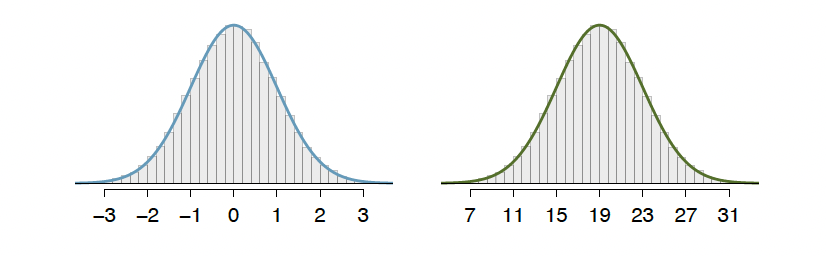
\includegraphics[width=0.8\textwidth]{normal1.png}
\caption{Standard Normal Distribution (Left) and a Non-standard Normal Distribution (Right)}\label{interpfig}
\end{figure}


\section{Confidence Intervals for Means} 
\subsection{Motivating Analogy} 
Consider spear fishing as distinct from net fishing.  Spear fishing is an all-or-nothing endeavor and requires the utmost precision.  If the fisherman is off by even the slimmest of margins, they return empty handed.  In short, the tip of the spear does not allow for much in the way of what we might call wiggle room.  Contrast this with net fishing where to come up with a fish, one only need to get the net in the general vicinity of the fish.  Moreover, the wider the net, the more imprecise one can be and still have a successful fishing trip.  

For the sake of this lecture, I want you to keep spear fishing in the back of your mind as the analogy to point estimation.  Point estimation can be thought of like the tip of the spear -- very precise but also very unforgiving.  That is, there is no wiggle room in a point estimate.  If you are off by even the slightest of margins, you have missed the parameter\footnote{Future classes will discuss just how unlikely it is that for a continuous variable, a point estimate is actually ever \textit{exactly} equal to the parameter of interest.  For our purposes, just consider Andy to be the spear fisherman in question and know he is incredibly inept at fishing.}.  By contrast, keep net fishing in the back of your mind as the analogy to interval estimation.  Compared to point estimation interval estimation allows for some wiggle room in attempting to estimate the true parameter of interest.  Much like a net, if we are willing to cast our interval wider and wider, we can be more confident that the interval actually includes the true parameter of interest (that we come up with a fish).  Hence, we will see there to be an inherent trade-off between precision and confidence within confidence intervals.  

\subsection{Defining a Confidence Interval} 

With the above motivating analogy in the back of our mind, consider the following general form of a confidence interval: 

\begin{center}
point estimate$\pm$ margin of error.  
\end{center}

The upshot here is that we take our single number best guess, the point estimate, and surround it with some wiggle room.  In the same way, we would not expect that a net fisherman would just arbitrarily run their net through any body of water.  Instead they would likely run it through the same vicinity that a spear fisherman would, only now the net fisherman has some margin of error available.  

The follow up question should be, ``what is this margin of error?"  It turns out that this is a product of a) how confident we want to be in the interval (what we will call a \textit{critical value}) and b) how much variability we expect in the estimator (what we will call \textit{standard error}).  Thus, we need to know where this critical value is coming from and what the standard error is.  

\textit{The Central Limit Theorem}: for sufficiently large samples ($n\geq 30$) of independent observations: 

\begin{center} 
$\bar{X} \sim N(\mu, \sigma/\sqrt{n})$.
\end{center}
What is this theorem really saying?  The sampling distribution\footnote{Ideally, this is a concept covered in a lecture on point estimation preceding the current lecture.} of $\bar{X}$ is approximately normal, centered around the right thing (the population mean) with a particular standard error.  Now, notice that the standard error has a population quantity in it, $\sigma$ the population standard deviation.  We rarely know this quantity, just as we rarely know the population mean.  In which case, we will use the next best thing -- the sample standard deviation, $S$.  

In which case, our $95\%$ confidence interval for $\mu$ is:

\begin{equation} 
\bar{x} \pm 1.96\frac{s}{\sqrt{n}}.
\end{equation} 
\textit{Remark}: We should emphasize that $1.96$ is the critical value associated with this interval, and it is only applicable under the conditions that we have a sufficiently large sample size and a $95\%$ confidence interval.  We will see this generalized in what follows, but for now, just think of this as being a metric of how confident we are in the given interval.  

\textit{Example 1}: 
I \textit{randomly sample} 100 Skidmore students and ask how many hours they study per week.  Summary statistics are as follows: \\

\begin{table}[ht]
    \centering
    \begin{tabular}{ccccc}
        \toprule
        n & $\bar{x}$ & s & min & max \\
        \midrule
        100 & 15.1 & 3.1 & 3.0 & 25.0 \\
        \bottomrule
    \end{tabular}
    \caption{Summary Statistics}
    \label{tab:summary}
\end{table}
Compute the $95\%$ confidence interval for $\mu$, the population mean time spent studying.\\ 
 \textit{\color{blue}{Answer: $\bar{x} \pm 1.96\frac{s}{\sqrt{n}} \Rightarrow$ $15.1\pm 1.96(\frac{3.1}{\sqrt{10}}) \approx [14.4924, 15.7076].$ }}

\subsection{Interpreting a Confidence Interval} 

The all important question becomes, how does one interpret such a confidence interval.  I would recommend the following, ``We are $95\%$ confident that the true parameter of interest, $\mu$, lies in the interval $[14.4924, 15.7076]$."  In short, we need to be very careful how we interpret such an interval, as there are several similar but subtly mistaken interpretations.  Let's discuss two.  

\begin{enumerate}
\item ``We are $95\%$ confident that the true parameter of interest, $\bar{x}$, lies in the interval $[14.4924, 15.7076]$".  The interval should always be a statement about the parameter, not the statistic.  In fact, we \textit{know} that the statistic is in the interval.  By construction, it is the midpoint.  What we are concerned with is whether the unknown $\mu$ is in said interval.  
\item ``The probability that $\mu$ is in the interval $[14.4924, 15.7076]$ is $0.95$".  The language of a probability can tend to obscure what is random and what is fixed in the above interval, and was one of the reasons for the review in Section \ref{rev}.  Indeed, $\mu$ is fixed and the interval(s) change with different samples.  Again, this is because the interval is based on sample quantities which themselves fluctuate from sample to sample.  Therefore, what we mean when we say ``We are $95\%$ confident that the true parameter of interest, $\mu$, lies in the interval $[14.4924, 15.7076]$" is that if we were to repeatedly sample from the population a large number of times and compute the corresponding $95\%$ confidence intervals, roughly $95\%$ of these (changing) intervals would contain the one (constant) parameter.  Figure \ref{ci} illustrates this with simulated confidence intervals and a known parameter of interest.  

\begin{figure}[h]
\centering
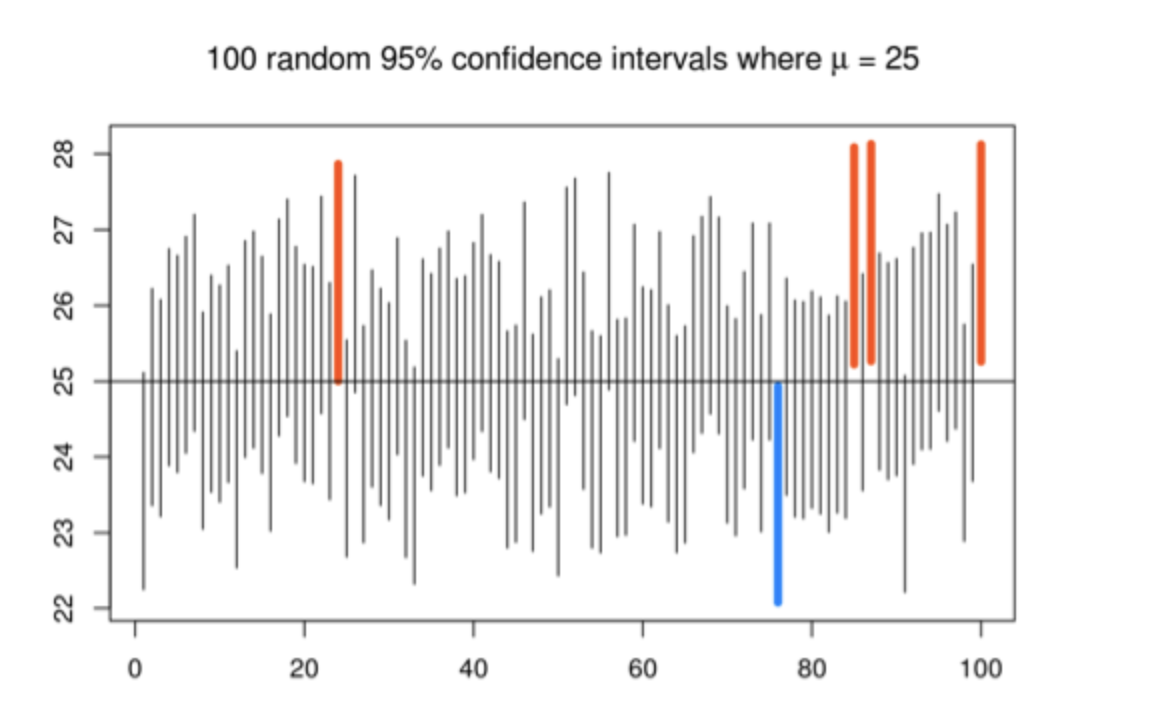
\includegraphics[width=0.8\textwidth]{ci.png}
\caption{$95/100$ intervals contain the one true parameter}\label{ci}
\end{figure}

\end{enumerate}

\subsection{Widening the Interval} 

What if we want to be more confident in the confidence interval?  We need a wider interval.  Analogously, if we wanted to be more sure that we came up with a fish, if we fished in the exact same spot with the exact same skill, we should use a wider net.  This will give us more margin of error.  

Again, for independent observations from a sufficiently large sample size, the $99\%$ confidence interval for $\mu$ is:

\begin{equation} 
\bar{x} \pm 2.58\frac{s}{\sqrt{n}}.
\end{equation}
\textit{Remark}: Notice that to increase the confidence (assuming the same data) we just widen the interval by using a larger critical value.  This is what was meant by the critical value being a measure of how confident we want to be in the interval.  Moreover, this large critical value is not just chosen as some arbitrary number larger than $1.96$.  Indeed, the critical value for a $99\%$ confidence interval for means (with sufficiently large sample size) is the number such that $99\%$ of normally distributed data falls within that many standard deviations of the mean.  That is, $99\%$ of normally distributed data falls within $2.58$ standard deviations of the mean, and $95\%$ falls within $1.96$\footnote{Critical values would likely be covered in a lecture on the normal distribution, but it is likely worthwhile to review them here.}.  

\textit{Example 2}: 
Compute the $99\%$ confidence interval for $\mu$, the population mean time spent studying in Example 1 above.   Summary statistics are in Table \ref{tab:summary2}.  

\begin{table}[ht]
    \centering
    \begin{tabular}{ccccc}
        \toprule
        n & $\bar{x}$ & s & min & max \\
        \midrule
        100 & 15.1 & 3.1 & 3.0 & 25.0 \\
        \bottomrule
    \end{tabular}
    \caption{Summary Statistics}
    \label{tab:summary2}
\end{table} 
 \textit{\color{blue}{Answer: $\bar{x} \pm 2.58\frac{s}{\sqrt{n}} \Rightarrow$ $15.1\pm 2.58(\frac{3.1}{\sqrt{10}}) \approx [14.3002, 15.8998].$ }}
 \textit{Remark:} Notice that the new interval is wider than the previous interval.  More than that, our $95\%$ confidence interval is completely contained within the $99\%$ confidence interval for the same sample.  The upshot is, if we want to be more confident that our interval contains the true parameter, widen the interval.  It makes the interval less specific or precise (in the sense that we have a wider range of possible values for $\mu$), but we can be more confident that $\mu$ is actually in that interval.  
 
 \textit{Question}:  How would the $90\%$ confidence interval for the same data relate to the $95\%$ and $99\%$ confidence intervals?\\
  \textit{\color{blue}{Answer: More narrow.  Completely contained within each of the above.}}
 
 \textit{Ticket-out-of-the-door}: We have now talked about the $90\%$, $95\%$, $99\%$ confidence intervals.  What would be required (conceptually) to have a $100\%$ confidence interval?\\
 \textit{\color{blue}{Answer: $[0,\infty]$.  We would have our interval include all possible values for a mean number of hours spent studying.  We have now sacrificed all precision in deference to complete confidence.  If you could imagine fishing with a net that covered the entire body of water, you could be certain to come up with a fish (probably multiple), but it would say absolutely nothing about your ability as a fisherman.}}

\section{Preview} 

The next two (hypothetical) lectures would likely address the following two questions:

\begin{enumerate} 

\item What happens if $n$ is small?  In particular, if $n<30$, what happens to the Central Limit Theorem and our critical values?  How do we compute confidence intervals in this case?\\
\textit{\color{blue}{Answer: Introduction of the Studentized-T Distribution.}}
\item What happens if I came to Skidmore with a preconceived belief that $\mu = 12$.  Do we have a way of assessing if I was wrong?  Otherwise put, is $15.1$ far enough away from $12$ that I can claim $\mu \neq 12$?\\
\textit{\color{blue}{Answer: Enter hypothesis testing!}}


\end{enumerate} 

\end{document}

